% Chapter 1

\chapter{Introduction} % Main chapter title

\label{Chapter1} % For referencing the chapter elsewhere, use \ref{Chapter1} 

%----------------------------------------------------------------------------------------

% Define some commands to keep the formatting separated from the content 
\newcommand{\keyword}[1]{\textbf{#1}}
\newcommand{\tabhead}[1]{\textbf{#1}}
\newcommand{\code}[1]{\texttt{#1}}
\newcommand{\file}[1]{\texttt{\bfseries#1}}
\newcommand{\option}[1]{\texttt{\itshape#1}}

%----------------------------------------------------------------------------------------
Dans cette partie, je donne une brève description du sujet de mémoire que j'ai développé tout au long de cette année.

Mon sujet s'intitule : Intégration de comportements humains dans les systèmes autonomes.

Je m'explique, nous connaissons en notre temps un très fort essor de nouvelles technologies de tous genres, celles-ci ont des buts divers et variés, que ce soit pour nous aider à choisir une playlist musicale afin de bien démarrer une journée de travail, ou encore pour nous aider à mieux gérer notre entreprise avec des logiciels dédiés,  jusqu'aux applications les plus compliquées dans le domaine médical tel que l'assistance d'un chirurgien lors d'une opération risquée.

Parmi les technologies les plus avancées et les plus prometteuses on trouve les intelligences artificielles, ces machines auxquelles on apprend à apprendre.

Celles-ci sont capable de mémoriser une quantité de données très élevée afin de cerner leurs environnements et ainsi pouvoir agir efficacement dans le but d'aider les hommes.

On les trouve partout, au supermarché, à la banque, sur internet, dans les jeux 
vidéo etc.

Malheureusement, malgré toute leur puissance de calcul, celles-ci ne sont pas capables de comprendre et d'interpréter une chose élémentaire qui fait le propre de l'homme: ses sentiments.

En effet, les IA actuelles peuvent résoudre des problèmes très complexes, mais sans savoir ce qu'engendrent leurs prises de décisions sur le ressenti de l'homme et sa moralité, pourront-elles vraiment nous être bénéfiques ? Ou au contraire: destructrices.

C'est la question à laquelle j'essaye de répondre lors de ce mémoire en appliquant ce principe aux intelligences artificielles que l'on peut trouver dans les jeux vidéo. Essayer de leur inculquer non seulement ce qui les entoure, mais aussi ce qu'implique de prendre telle ou telle décision et ses répercussions sur l'homme, ou en l'occurrence dans mon cas, le joueur.

L'objectif est donc d'utiliser des androrithmes \parencite{humanityvstechnology} ( algorithmes calqués sur le modèle humain et nourris par ce dernier ) et de les appliquer à différentes intelligences artificielles dans des jeux vidéo open-source. 



\section{Prérequis}

L'idée qu'un jour les robots puissent avoir des émotions a capturé l'imagination de beaucoup et a été dramatisée par des robots et des androïdes dans de nombreux films de science-fiction. Ce mémoire aborde la question de savoir si les robots peuvent prendre des décisions qui ne sont pas liées à un choix rationnel, ce qui supposerait que ceux-ci agissent sous le feu de l’émotion. Les études sur le cerveau et notamment sur  les émotions reposent principalement sur l’étude des aspects sociaux, communicatifs, adaptatifs, régulateurs et expérientiels de celles-ci, ainsi la neurochimie révèle la manière dont différents «neuromodulateurs» tels que la sérotonine, la dopamine et les opioïdes peuvent affecter l’équilibre émotionnel du cerveau et les études de différentes régions telles que l'amygdale et le cortex orbifrontal fournissent une vue du cerveau comme un réseau de sous-systèmes en interaction. \parencite{whoneedsemotions}


%----------------------------------------------------------------------------------------

\subsection{ L'amygdale}

L'amygdale (latin, corpus amygdaloideae) [Figure \ref{fig:amy}, Page \pageref{fig:amy}]
est un ensemble de neurones en forme d'amande situés au plus profond du lobe temporal médial du cerveau.
L'amygdale, qui joue un rôle clé dans le processus des émotions, fait partie du système limbique.
Chez les humains et les autres animaux, cette structure cérébrale sous-corticale est liée à la fois aux réactions de peur et au plaisir.
Sa taille est en corrélation positive avec le comportement agressif d'une espèce à l'autre.
Tels que l'anxiété, l'autisme, la dépression, le trouble de stress post-traumatique et les phobies sont soupçonnés d'être liés au fonctionnement anormal de l'amygdale, en raison de dommages, de problèmes de développement ou d'un déséquilibre neurotransmetteur.

\begin{figure}[th]
\centering
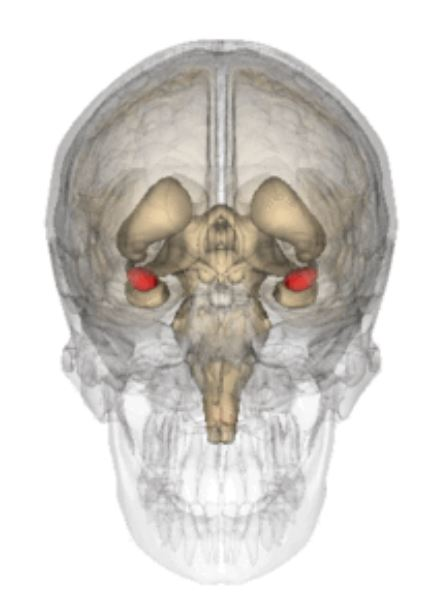
\includegraphics{Figures/2}
\decoRule
\caption[L'amygdale]{Vue 3D de l'amygdale (en rouge).}
\label{fig:amy}
\end{figure}


\subsection{Le cortex orbitofrontal (OF)}

Le cortex orbifrontal [Figure \ref{fig:cortex}, Page \pageref{fig:cortex}] est une région du cortex cérébral qui entre en jeu dans le processus de décision. Il est situé en position antérieure et sur la face inférieure du cortex préfrontal. Il prend son nom des lobes frontaux et du fait qu'il est situé au-dessus des orbites.


Cette partie du cortex préfrontal est en connexion avec le thalamus. Parce qu'il est actif dans les émotions et le système de récompense, le cortex orbitofrontal est souvent considéré comme faisant partie du système limbique.\parencite{cortex}

\begin{figure}[th]
\centering
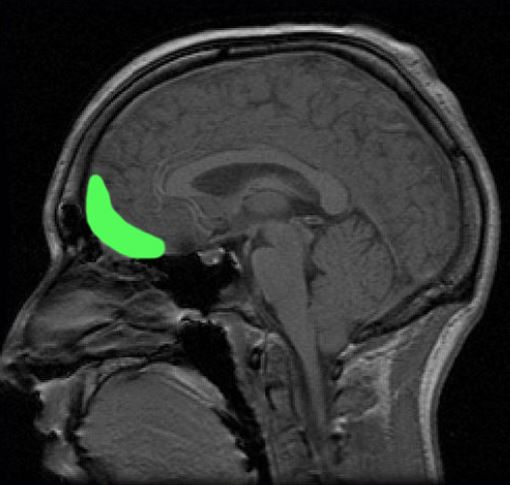
\includegraphics{Figures/3}
\decoRule
\caption[Cortex Orbifrontal]{Emplacement approximatif de cortex orbitofrontal.}
\label{fig:cortex}
\end{figure}


\subsection{Émotions}

Chez les êtres humains, l'émotion inclut fondamentalement « un comportement physiologique, des comportements expressifs et une conscience » \parencite{myers2004theories}

~\par
Il existe certaines catégories des émotions :

\begin{itemize}
\item émotions « cognitives » par opposition aux émotions « non cognitives »
\item émotions instinctives (des amygdales), par opposition aux émotions cognitives (du cortex orbitofrontal)
\item émotions primaires et secondaires
\end{itemize}

~\par

\begin{figure}[th]
\centering
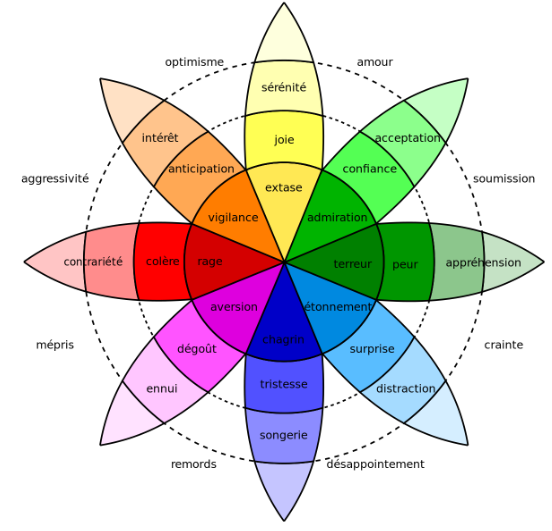
\includegraphics{Figures/emotions.PNG}
\decoRule
\caption[Roue des émotions de Robert Plutchik]{Roue des émotions de Robert Plutchik}
\label{fig:roue}
\end{figure}


\begin{quotation}

 "La théorie psycho-évolutionniste des émotions de Robert Plutchik \parencite{plutchik} est l'une des méthodes de classification des réactions émotives générales. Plutchik considérait qu'il y avait huit émotions de base [Figure \ref{fig:roue}] : la joie, la peur, le dégoût, la colère, la tristesse, la surprise, la confiance et l'anticipation. Un professeur et psychologue américain Robert Plutchik propose ses 4 émotions fondamentales primaires (la peur, la colère, la joie, la tristesse), qui s'associent à des mécanismes de mémoire et de réflexion pour donner 4 autres émotions fondamentales secondaires (la confiance (liée à la joie), le dégoût (lié à la tristesse), l'anticipation (liée à la colère) et la surprise (liée à la peur)), dont les fonctions respectives seraient la préservation, la protection des acquis, la reproduction, la réintégration, l'incorporation, le rejet, l'orientation et l'exploration). D'autres systèmes de classement des émotions, comme celui de Paul Ekman, ne considèrent que 4 à 6 émotions primaires au lieu de 8, car dans la mesure où les émotions combinées font intervenir des mécanismes de réflexion et de mémoire (par exemple la confiance est liée à un ensemble de souvenirs joyeux) voire de pensée abstraite, il ne s'agit plus d'émotions mais de sentiments par définition.

~\par
Plutchik a organisé ses émotions en paires d'opposés : la joie et la tristesse, la peur et la colère, le dégoût et la confiance, la surprise et l'anticipation. Il faut bien garder à l'esprit que chacune de ces émotions peut varier en intensité, ce qui génère un grand nombre de mots pour les décrire. Par conséquent, il y combine l'idée d'un cercle des émotions et celle d'une palette de couleurs pour représenter cette variation d'intensité et la classer en niveaux, même si la séparation entre les niveau n'est pas franche. Comme ces dernières, les émotions de base peuvent s'exprimer à divers degrés d'intensité et se combiner l'une à l'autre pour former des émotions différentes. C'est ainsi que Plutchik est venu à définir les dyades primaires [Figure \ref{fig:TbEm}, Page \pageref{fig:TbEm}] (combinaisons de deux émotions de base adjacentes), secondaires (combinaisons d'émotions de base voisines à une émotion près) et tertiaires (combinaisons d'émotions de base voisines à deux émotions près) qui suivent   \parencite{tayari2009modelisation} : "

\end{quotation}


\begin{figure}[th]
\hspace*{-1.9cm} 
\centering
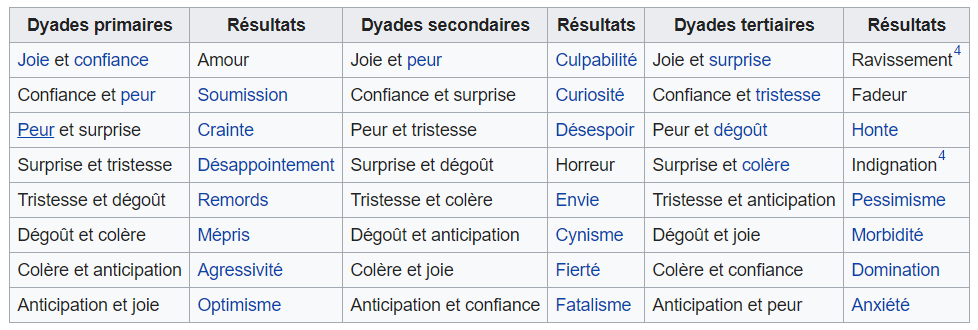
\includegraphics{Figures/tableauEmotions.PNG}
\decoRule
\caption[Tableau de la théorie de Plutchik]{Dyades primaires, dyades secondaires, dyades tertiaires et leurs résultats selon la théorie de Plutchik}
\label{fig:TbEm}
\end{figure}




